\documentclass{article}
\usepackage[colorlinks=true]{hyperref}
\usepackage{pdfpages}

%\usepackage{titling}
%\setlength{\droptitle}{-10em}
%\usepackage{fullpage}

\title{Database Systems: Final Project Proposal}
\author{Mark Hudnall \and Sam Konowitch}
\date{April 2012}
\begin{document}
    \maketitle
    \section*{Domain}
    For our final project, we hope to tackle the domain of athletics software. In particular, 
    we wanted to provide a fitness tracking web application for sports teams. We want to expand 
    our initial fitness tracking vision to fully model a sports team hierarchy (including 
    positions, captains, and coaches). We plan to provide specialized views for coaches, 
    athletes on a team, and independent athletes (not in a sport, but wanting to track fitness 
    regardless) that provide the relevant information for each role in a digestible way. 

    \section*{Key Features}
    At the base of our application, we hope to provide an easy, web-based system for tracking 
    fitness and workouts. For coaches and athletes, we hope to model a team as close to reality 
    as possible, including relevant team information like positions and captains. Coaches and 
    captains will be able to set workouts for the week, while players can log their progress 
    and view summary statistics. If we have extra time, we hope to expand our fitness tracking 
    and team modeling to include in game statistics, which would be sport specific. We also 
    hope to provide support for professional athletes, who have contracts and receive salaries. 

    \section*{Expected Results}
    By the end of the project, we hope to present a polished web application. The web 
    application will provide a login system. Coaches register and add players, or players 
    can register as independents. Coaches and captains will have an interface to specify 
    required workouts. Players will be presented with a view of upcoming and previous workouts. 
    Players can log their own progress, as well as view the progress of other members of the 
    team (a team cannot view another team’s progress). Coaches will be able to designate “roles”
    for players on his/her team, like positions or captain status. This will determine what 
    information players can view in the webapp. 

    \section*{Tentative Schedule}
    \begin{tabular}{l || l | l}
        Date & Goal & Status \\
        \hline
        April 2 & ER Diagrams finalized & completed \\ 
        April 6 & Relations finalized & completed \\ 
        April 9 & Normalization complete & completed \\ 
        April 11 & {\tt schema.sql} & completed \\ 
        \textbf{April 12} & Application scaffolded & completed \\ 
        April 20 & Generated Data & completed \\ 
        April 23 & Database Security and indexing & completed \\ 
        \textbf{April 26} & Front-end for Coach and Players complete & completed  \\ 
        \textbf{May 1} & App tested and feature complete & completed  \\ 
    \end{tabular}

    \section*{Technologies}
    We plan to use MySQL as our DBMS. We will be using Python as our server side language,
    for both web development and database interfacing (via the 
    \href{http://mysql-python.sourceforge.net/MySQLdb.html}{mysql-python} module). 
    We are currently planning to use the \href{http://flask.pocoo.org/}{Flask} web framework.
    We are both comfortable with Python, and the Flask framework is very easy to use, which
    will let us focus more on the database portion of the assignment. {\tt mysql-python } is
    essentially identical to {\tt JDBC}.

    \section*{ER Diagram}
    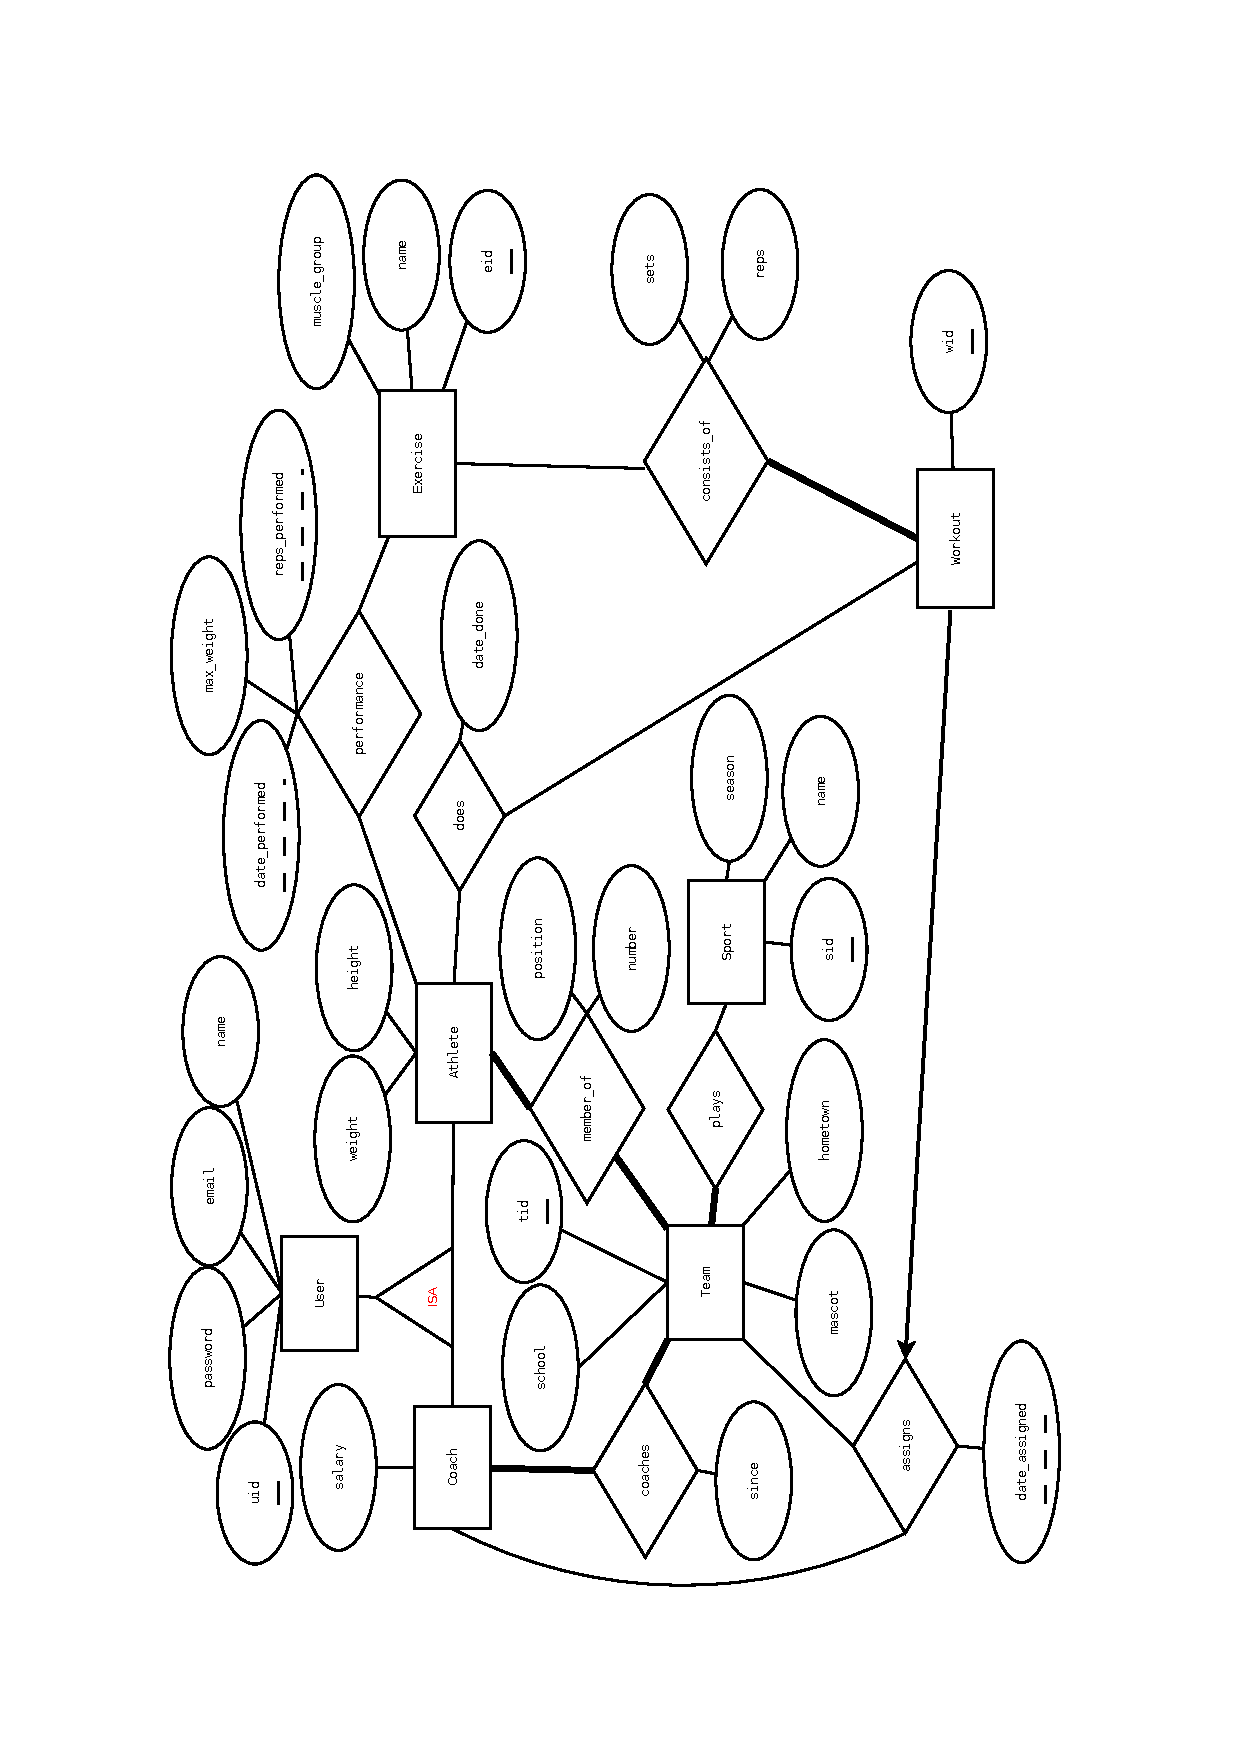
\includepdf{erdiagram.pdf}

    \section*{Relational Model}
    \begin{verbatim}
User(*uid, name, email, password)
Coach(*uid, salary)
Athlete(*uid, weight, height)
coaches(*uid, *tid, since)
Team(*tid, school, hometown, mascot)
Sport(*sid, name, season)
plays(*tid, *sid)
member_of(*uid, *tid, position, number)
Workout(*wid, uid, tid, *date_assigned)
Exercise(*eid, name, muscle_group)
consists_of(*wid, *eid, sets, reps)
assigns(*uid, *wid, *date_assigned)
does(*uid, *wid, date_done)
performance(*uid, *eid, *date_performed, *reps_performed, max_weight)
    \end{verbatim}
{\tt *} denotes a primary key.

\section*{Functional Dependencies and Normalization}

We chose to eliminate as much redundancy as possible in our database and thus chose to normalize our relations to BCNF.  We have identified three violations of BCNF in our relational model. 

First, let us consider the Team relation.  We observed that a team from a given school 
will have a given mascot (for instance, teams from ``Pomona-Pitzer'' will have the mascot
``Sagehen'', while the school ``UCLA'' will have the mascot ``Bruins'' for all its teams). Thus there is 
a functional dependency from school to mascot. Thus we decompose Team into two relations:
Team(tid, school, hometown) and TeamMascot(school, mascot). This eliminates the functional
dependency in Team. For TeamMascot, we have a FD from school $\to$ mascot, but since school
is a key, the relation is in BCNF. Thus both relations are in BCNF.

Next we consider the Sport relation. We observed that for the sports we deal with, the same 
sports are always in the same season. Thus there is a functional dependency from a sport's
name to its season. Thus we decompose Sport into two relations: Sport(sid, name) and 
SportSeason(name, season). This eliminates the FD in Sport. SportSeason has a FD from
name to season, but since name is a key, SportSeason is in BCNF. Thus both relations 
are in BCNF. 

Our final violation of BCNF is in the Exercise relation.  We have a functional dependency from name to muscle\underline{\hspace{2mm}}group because we have determined that any exercises with the same name will work the same muscle groups.  For example, "bench press" will always work "chest" and "squats" will always work "legs", so we need to decompose this relation to put it in BCNF.  The result of our decomposition will be two tables Exercise(eid, name) and ExerciseMuscles(name, muscle\underline{\hspace{2mm}}group), eliminating the FD in Exercise and moving it to ExerciseMuscles, where since name is a key, the relation is BCNF.

Thus our final set of relations is:
    \begin{verbatim}
User(*uid, name, email, password)
Coach(*uid, salary)
Athlete(*uid, weight, height)
coaches(*uid, *tid, since)
Team(*tid, school, hometown)
TeamMascot(*school, mascot)
Sport(*sid, name)
SportSeason(*name, season)
plays(*tid, *sid)
member_of(*uid, *tid, position, number)
Workout(*wid, uid, tid, *date_assigned)
Exercise(*eid, name)
ExerciseMuscles(*name, muscle_group)
consists_of(*wid, *eid, sets, reps)
does(*uid, *wid, date_done)
performance(*uid, *eid, *reps_performed, max_weight)
    \end{verbatim}

\section*{Interesting Features}

We have several interesting features as part of our application that we wanted to illuminate here.

\subsection*{Stored Procedure}
As a general rule, we tried as much as possible to move logic to the database level, rather than
the application level. One such example is the stored procedure we used to help calculate,
given a team id and workout id, which members of a team have completed a workout and which
have not. Here is the procedure:

\begin{verbatim}
CREATE PROCEDURE TeamProgress (
    IN tid INTEGER,
    IN wid INTEGER
)
BEGIN
    (SELECT M.uid, A.name, FALSE as completed
    FROM member_of M, User A
    WHERE M.tid = tid 
        AND M.uid = A.uid
        AND M.uid NOT IN (SELECT D.uid FROM does D WHERE D.wid=wid)
    )
    UNION
    (SELECT M.uid, A.name, TRUE as completed
    FROM member_of M, User A
    WHERE M.tid = tid 
        AND M.uid = A.uid
        AND M.uid IN (SELECT D.uid FROM does D WHERE D.wid=wid)
    );
END
\end{verbatim}

When the procedure is invoked, the resulting set of tuples that is returned 
looks something like:

\begin{verbatim}
mysql> CALL TeamProgress(1,1);
+-----+----------------------+-----------+
| uid | name                 | completed |
+-----+----------------------+-----------+
| 396 | Sylvester Norman     |         0 |
|  11 | Christopher Anderson |         1 |
|  46 | Henry Campbell       |         1 |
|  81 | Carlos Henderson     |         1 |
| 116 | Vincent Gibson       |         1 |
| 151 | Oscar Palmer         |         1 |
| 186 | Roberto Fox          |         1 |
| 221 | Ron Morrison         |         1 |
| 256 | Dwayne Holland       |         1 |
| 291 | Tracy Holt           |         1 |
| 326 | Angelo Lyons         |         1 |
| 361 | Alton Glover         |         1 |
| 431 | Drew Ballard         |         1 |
| 466 | Dexter Norton        |         1 |
+-----+----------------------+-----------+
14 rows in set (0.00 sec)
\end{verbatim}

This stored procedure provides a simple abstraction for our application code,
so instead of having to run the query and have complicated looking application code,
we simply call the stored procedure and act on the result. We use this 
procedure heavily for the coach workflow; a coach can quickly see which athletes
on a team have and have not completed a workout.

\subsection*{Integrity Constraints}

Our ER Diagram shows our initial hopes relating to key and participation constraints. 
We hoped to enforce: a team has at least one athlete, an athlete has at least one team,
a team plays at least one sport, and a workout is assigned by one and only one coach. 

We implemented the total participation and key constraint on workouts by merging the 
``assigns'' relationship with the ``Workout'' table. The other constraints proved 
trickier, however. We were hoping to use triggers to implement the first two 
constraints and ensure that they hold with checks, but we ran into a problem. 
When an athlete registers, the integrity constraint would mean he must also join 
a team. However, in order to join a team, the \verb,member_of, relation requires a 
foreign key to the ``User'' table. We could not figure out a way around this problem,
so we omitted the constraint from our schema. 

\subsection*{ISA}

In our ER Diagram, a ``User'' ISA Athlete or a Coach. We implemented this in our
schema with three separate tables. The ``User'' table contains a uid, name,
email address, and password. The ``Athlete'' table has a foreign key to ``User''
on uid, and additional fields for height and weight. The ``Coach'' table also
has a foreign key on uid and an additional field for salary. With our implementation,
we allow for Users who are neither Athletes nor Coaches, since we have a separate
table for Users.

\subsection*{Security Considerations}

Since we were storing passwords in the database, we did not want to store them
in plaintext, since if our database were compromised, the attacker could then
impersonate any user. Thus, we hashed and salted our passwords before storing them.
This was done using a built-in function of the Flask web framework. Thus,
a password like {\tt test1234}, when hashed and salted, was recorded in the
database as \verb, sha1$3EZTz7F7$8b2e64a891662a9c5431b6936c35f5740992a708,. 
Hashing itself adds security. However, only hashing leaves the database vulnerable
to attacks using rainbow tables, prebuilt tables that match a plaintext password
to its hash. By salting a password, prepending some string to the password before
it is hashed, we add an additional layer of security that makes it more difficult
to use rainbow tables (since one would need to construct a rainbow table with the salt
prepended to every plaintext password, a time consuming process).

\subsection*{Database Tuning}

As we built and tested our application, we realized that we were performing several
inefficient queries that would benefit from added indexes. In particular, when 
a coach builds a workout, we built the application so that the coach first chooses
a muscle group and then the corresponding exercises were shown. We then use
the exercise name to look up the exercise id from the ``Exercise'' table. 
In essence, we were actually using the table ``backwards'', using a field
to find the primary key. Both exercise names and ids are unique.

Our decompositions left ``Exercise'' with a foreign key on $name$ 
to ``ExerciseMuscles''. We thus added the {\tt UNIQUE} keyword to the $name$
field in ``ExerciseMuscles'', thus adding an implicit index on the field. This
means that queries on $name$ will be faster, improving database performance.

We also added the {\tt UNIQUE} keyword to the $email$ field of ``User''. 
Though it is easiest to refer to users by their ids in urls and queries, a 
user logs in using his or her email address. Since this is a frequently used
feature, we wanted to ensure that looking up a $uid$ given an email address
would be performant. 

\section*{Future Work}

As we said before, we did not implement all of our integrity constraints that we initially had in our ER diagram, so this would be the top priority for the future.  We would either implement this using triggers or by making changes to our schema.  There are also queries that we would want to improve the efficiency of our stored procedure. 

On the application side, we would want to give users more opportunities to input data, especially at registration.  Right now, there is no way to add a new team to the database and when players are added to the database, they do not get to choose their position or number.  Our database could easily handle such uses and we did not have time to set up the interface forms for adding this information to the database.


\section*{Documentation}

We have documented our code in the {\tt README} file, but we also wanted to add
those instructions here for posterity. 

\subsection*{Installation}

We assume that {\tt mysql} and {\tt >= python 2.6} are already installed on a 
OS X system. We tested our setup with both Lion and Snow Leopard. 

\begin{enumerate}
    \item
        Get {\tt pip}:
        \begin{verbatim}
        $ sudo easy_install pip
        \end{verbatim}

    \item
        Get {\tt virtualenv}:
        \begin{verbatim}
        $ sudo pip install virtualenv
        \end{verbatim}

    \item
        Get {\tt virtualenvwrapper}. It makes using {\tt virtualenv} easier:
        \begin{verbatim}
        $ sudo pip install virtualenvwrapper
        \end{verbatim}

    \item
        Add this to your {\tt .bashrc} or run in your terminal:
        \begin{verbatim}
        source /usr/local/bin/virtualenvwrapper.sh
        \end{verbatim}

    \item 
        In the terminal, make a `virtualenv` for this project:
        \begin{verbatim}
        $ mkvirtualenv database-final
        \end{verbatim}

    \item 
        You should automatically be working in the environment. In your shell,
you should see something like:
        \begin{verbatim}
        (database-final) $ 
        \end{verbatim}
        If you don't, then you can enter a virtual environment by running:
        \begin{verbatim}
        $ workon database-final
        \end{verbatim}
        ``database-final'' is just the name of the virtualenv you created.

    \item To install the required dependencies for this project in one fell swoop,
        {\tt cd} to the project root and then run:
        \begin{verbatim}
        (database-final) $ pip install -r requirements.txt
        \end{verbatim}

    \item Now, let's populate our database. In the {\tt data} folder, there 
        is a file called {\tt all.sql}, which containts both the schema and 
        all generated data we used. In the project root:
        \begin{verbatim}
        (database-final) $ cd data
        (database-final) $ mysql
        mysql> source all.sql
        \end{verbatim}

    \item The database should now be populated. Now back in the project root,  run the server:
        \begin{verbatim}
        (database-final) $ python app.py
        * Running on http://127.0.0.1:5000/
        \end{verbatim}

    The server should now be running on port 5000.
\end{enumerate}


\subsection*{Overview of Included Files}

In the project root, we have a {\tt README} with instructions for setting up the server. 
The actual server code is contained in {\tt app.py}. Settings for the server, including
the database name, host, username, and password are in {\tt settings.py}. 

We also have several folders. {\tt static} and {\tt templates} are part of the server.
{\tt static} contains static resources like images, javascript code, and css. For our
server, we used a UI framework called \href{http://twitter.github.com/bootstrap/}{Twitter Boostrap}. 
The {\tt templates} folder contains various html templates used by our server. Flask
templates are similar to JSPs, except that most of the application logic is done in {\tt app.py}.
Variables can be passed to templates and templates have limited control flow features like
{\tt for} loops and {\tt if} statements. 

The {\tt data} folder contains various scripts and text files we used for generating
our data. We have concatenated the result of running all the scripts into {\tt all.sql},
but they are available for your perusal. The {\tt docs} folder contains our final
write-up, progress reports, and other documentation, like our ER diagram. 

\end{document}


